% !TeX spellcheck = es_ES
\documentclass[12pt, titlepage]{article}
\usepackage[nottoc,notlot,notlof,numbib]{tocbibind}
\usepackage[letterpaper, margin=2.5cm]{geometry}
\usepackage[utf8]{inputenc}
\usepackage[spanish]{babel}
\usepackage{listings}
% imagenes
\usepackage{graphicx} 
\usepackage{float}
% fin imagenes
\usepackage{url}
\usepackage{color}
\usepackage{amsmath}
\usepackage{bm}

\definecolor{dkgreen}{rgb}{0,0.6,0}
\definecolor{gray}{rgb}{0.5,0.5,0.5}
\definecolor{mauve}{RGB}{253,151,31}
\definecolor{deepred}{RGB}{249,38,114}

\lstset{frame=tb,
	language=MATLAB,
	aboveskip=3mm,
	belowskip=3mm,
	showstringspaces=false,
	columns=flexible,
	numbers=left,
	stepnumber=1,
	basicstyle={\small\ttfamily},
	numberstyle=\tiny\color{gray},
	keywordstyle=\color{blue},
	commentstyle=\color{dkgreen},
	stringstyle=\color{mauve},
	breaklines=true,
	breakatwhitespace=true,
	tabsize=2,
	morekeywords={self, append},
	emph={},
	emphstyle=\color{deepred}
}

\title{Reporte}
\author{Barrera Pérez Carlos Tonatihu \\ Profesor: Moreno Armendariz Marco Antonio \\ Redes Neuronales \\ Grupo: 3CM2 }
\begin{document}
    \maketitle
    \tableofcontents
    \newpage
    %\section{Introducción}
El objetivo del siguiente trabajo es sentar las bases de los principales puntos 
en el estudio del Perceptrón Multicapa (Multilayer Perceptron) entre los que 
están sus características, las partes que lo conforman y el como estas partes 
trabajan juntas para lograr el funcionamiento que el MLP presenta. Conociendo 
su funcionamiento se puede determinar cuales son las principales actividades en 
las que es empleada esta arquitectura de redes neuronales lo cual, a su vez, 
explica el porque dicha red es de tal importancia en el campo de las redes 
neuronales.
\\\\
Sin embargo, todo este conocimiento teórico seria nada si no se ve aplicado a 
algún problema en especifico, es debido a esto que en esta práctica se empleo 
el perceptrón multicapa para realizar la aproximación de señales (la cual es 
una de las principales aplicaciones que tiene esta red) esta aproximación fue 
desarrollada utilizando la herramienta MATLAB, entre las principales 
características que tiene el programa desarrollado están.
\begin{itemize}
 \item Entrada de datos por parte del usuario.
 \item Distintos métodos para determinar la convergencia de la red.
 \item Graficación de los resultados obtenidos por el perceptrón.
\end{itemize}
Aunado a esta implementación se encuentra la discusión de resultados en la cual 
se realiza un análisis de los datos obtenidos de los resultados 
experimentales con distintos casos de pruebas. Al hacer dicho análisis se llego 
a diferentes conclusiones respecto a la implementación realizada y en generar a 
la red neuronal utilizada como es el caso de sus ventajas y las limitaciones 
que tiene el uso de esta.
    %\section{Marco teórico}
Además de presentar la teoría relacionada con el MLP es necesario explicar lo que es el algoritmo de propagación hacia atrás (o Backpropagation en inglés) que es la base del aprendizaje de esta arquitectura.

El perceptrón multicapa (Multilayer Perceptron) surge de la necesidad de tratar problemas que no son linealmente separables es por esto que Frank Rosenblatt y Bernard Widrow propusieron redes multicapa pero no pudieron generalizar los algoritmos necesarios para entrenar dichas redes.

Dicho algoritmo fue descrito hasta 1974 por Paul Werbos pero fue hasta 1980 cuando se empezó a divulgar y fue entonces cuando el MLP entrenado por el algoritmo de backpropagation se ha convertido en la red neuronal más utilizado. \cite{libro1}
\subsection{Perceptron multicapa}
Un perceptron multicapa es aquello en el cual la salida de una capa es la entrada de la siguiente capa, un ejemplo de esto es el mostrado en la figura \ref{fig:MLP} donde se presenta un MLP de tres capas. En un MLP cada capa puede tener diferente número de neuronas y distintas funciones de transferencia. Para poder diferenciar cada capa se utiliza un superindice como por ejemplo:
\[ \begin{bmatrix} R & S^1 & S^2 & S^3 & \dots & S^N \end{bmatrix} \]

\begin{figure}[H]
    \begin{center}
        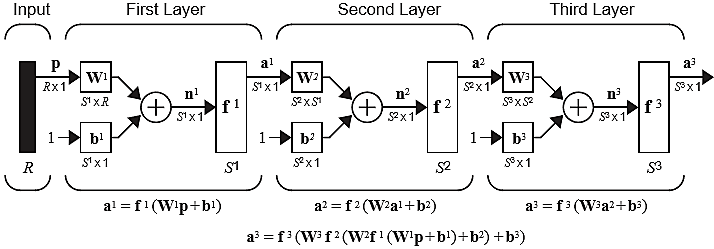
\includegraphics[width=16cm]{img/MLP.png}
        \caption{Perceptron de tres capas. \cite{libro1}}
        \label{fig:MLP}
    \end{center}
\end{figure}

En donde $S^1$ indica el número de neuronas de la capa uno, $S^2$ el número de neuronas en la capa dos y así consecutivamente. Esta misma estructura permite identificar la arquitectura de la red neuronal donde $R$ es el número de entradas. Para identificar el conjunto de funciones que se utiliza en cada capa se utiliza.

\[ \begin{bmatrix} F^1 & F^2 & F^3 & \dots & F^N \end{bmatrix} \]


Cada uno de estos elementos hace referencia alguna función de activación, las funciones que más se suelen utilizar son no lineales algunas de estas son.

\begin{itemize}
    \item Log-Sigmoid
    \[ a = \dfrac{1}{1+e^{-n}}\]
    \item Hyperbolic Tangent Sigmoid
    \[ a = \dfrac{e^n - e^{-n}}{e^n + e^{-n}}\]
    \item Linear
    \[ a = n\]
\end{itemize}

\begin{figure}[H]
    \begin{center}
        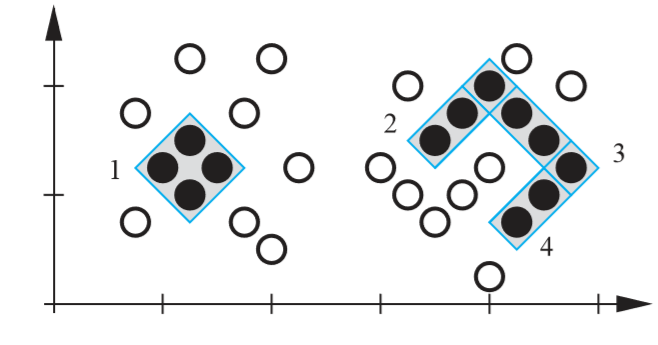
\includegraphics[width=7cm]{img/patrones.png}
        \caption{Clasificación de patrones. \cite{libro1}}
        \label{fig:clasificacion}
    \end{center}
\end{figure}

Las principales aplicaciones del MLP son:
\begin{itemize}
    \item Clasificación de patrones, objetos y caracteres como en la figura \ref{fig:clasificacion}.
    \item Aproximación de funciones.
    \item Compresión y codificación de información
    \item Reconocimiento de palabras (véase figura \ref{fig:palabras}).
    \item Segmentación de imágenes \cite{pdf}.
\end{itemize}

\begin{figure}[H]
    \begin{center}
        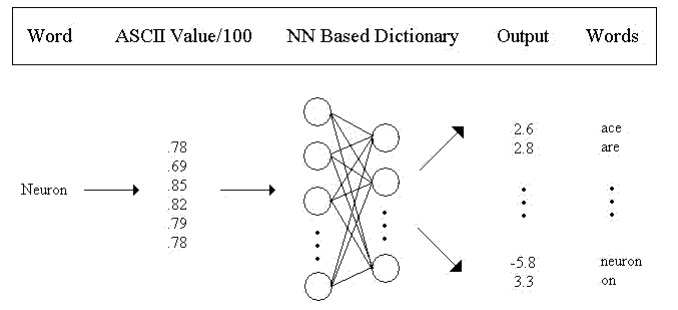
\includegraphics[width=12cm]{img/palabras.png}
        \caption{Diagrama del reconocimiento de palabras. \cite{pdf}}
        \label{fig:palabras}
    \end{center}
\end{figure}

La aproximación de señales se usa en sistemas de control en donde se trata de encontrar una función que pueda mapear mediciones de salidas a controles de entrada. Se puede realizar la aproximación de cualquier función si se tienen suficientes neuronas en las capas ocultas. 
\subsection{Backpropagation}
Para el estudio de backpropagation es importante conocer las ecuaciones que se usan en el aprendizaje que realiza. La primera de ellas está relacionada con las salidas de cada capa del MLP, estas ecuaciones son otra forma de representar la arquitectura de la figura \ref{fig:MLP}.

\begin{equation} \label{eq:1}
\boldsymbol{a}^0 = \boldsymbol{p}
\end{equation}
\begin{equation} \label{eq:2}
\boldsymbol{a}^{m+1} = \boldsymbol{f}^{m+1}(\boldsymbol{W}^{m+1}\boldsymbol{a}^{m}+\boldsymbol{b}^{m+1}
), \quad \text{Para $m=0, 1, \ldots M-1$}
\end{equation}
\begin{equation} \label{eq:3}
    \boldsymbol{a} = \boldsymbol{a}^{M}
\end{equation}
El valor de $M$ es el número de capas que tiene la red. La ecuación \ref{eq:1} hace referencia a que la capa uno tiene como entrada el conjunto de datos $\boldsymbol{p}$. Por otro lado la ecuación \ref{eq:3} es considerado como la salida final de la red neuronal.

El algoritmo backpropagation es una generalización del algoritmo LMS ya que ambos utilizan el error cuadrático medio, además utiliza un conjunto de entrenamiento compuesto por la entrada a la red y su correspondiente salida objetivo.
\[ \left\lbrace \boldsymbol{p_1}, \boldsymbol{t_1} \right\rbrace, \left\lbrace \boldsymbol{p_2}, \boldsymbol{t_2} \right\rbrace, \dots, \left\lbrace \boldsymbol{p_Q}, \boldsymbol{t_Q} \right\rbrace  \]
El objetivo de utilizar el una entrada y un target es utilizar un algoritmo de aprendizaje y con ello minimizar el error de salida de la red, dicho error es calculado con la siguiente formula.
\[ F(\boldsymbol{x}) = E \left[ \boldsymbol{e}^{T}\boldsymbol{e} \right] = E \left[ (\boldsymbol{t-a})^{T}(\boldsymbol{t-a}) \right]  \]
Aquí, $\boldsymbol{x}$ es el vector de pesos y bias de la red. Para una iteración (la propagación de un dato) esta ecuación se convierte en.
\[ \hat{F} (\boldsymbol{x}) = E \left[ \boldsymbol{e}^{T}\boldsymbol{e} \right] = E \left[ (\boldsymbol{t-a})^{T}(\boldsymbol{t-a}) \right]  \]
Esto hace que el algoritmo de gradiente descendente para pesos y bias sea.
\begin{equation} \label{eq:4}
w_{i, j}^{m}(k+1) = w_{i, j}^{m}(k) - \alpha \frac{\partial \hat{F}}{\partial w_{i, j}^{m}}
\end{equation}

\begin{equation} \label{eq:5}
b_{i}^{m}(k+1) = b_{i}^{m}(k) - \alpha \frac{\partial \hat{F}}{\partial b_{i}^{m}}
\end{equation}

Para poder trabajar con estas ecuaciones se debe de utilizar la regla de la cadena para facilitar el calculo de las derivadas parciales. Esto produce que se definan nuevos elementos los cuales son las sensitividades de $\hat{F}$ para cada elemento en cada capa de la red, dichas sensitividades producen los siguientes cambios.
\begin{equation} \label{eq:6}
\frac{\partial \hat{F}}{\partial w_{i, j}^{m}} = s_{i}^{m}a_{j}^{m-1}
\end{equation}
\begin{equation} \label{eq:7}
\frac{\partial \hat{F}}{\partial b_{i}^{m}} = s_{i}^{m}
\end{equation}
Al remplazar \ref{eq:6} y \ref{eq:7} en las ecuaciones \ref{eq:4} y \ref{eq:5} respectivamente y generalizando dichas ecuaciones a toda la matriz de pesos y bias para cada capa obtenemos las siguientes expresiones.

\begin{equation} \label{eq:8}
\boldsymbol{W}^{m}(k+1) = \boldsymbol{W}^{m}(k) - \alpha \boldsymbol{s}^{m} (\boldsymbol{a}^{m-1})^T
\end{equation}

\begin{equation} \label{eq:9}
\boldsymbol{b}^{m}(k+1) = \boldsymbol{b}^{m}(k) - \alpha \boldsymbol{s}^{m}
\end{equation}
Ahora lo importante es definir $\boldsymbol{s}^{m}$ para cada capa $\boldsymbol{m}$ de la red neuronal. Para la ultima capa del perceptrón, la capa $\boldsymbol{M}$ la sensitividad queda definida como:
\begin{equation} \label{eq:10}
    \boldsymbol{s^M} = 
    -2\boldsymbol{\dot{F}^{M}}(\boldsymbol{n^{M}})(\boldsymbol{t-a})
\end{equation}
Mientras que para el resto de las capas la sensitividad es:
\begin{align*}
\boldsymbol{s}^M &= 
-2\boldsymbol{\dot{F}}^{M}(\boldsymbol{n}^{M})(\boldsymbol{t-a}) \\
\boldsymbol{s}^{m} &= 
\boldsymbol{\dot{F}}^{m}(\boldsymbol{n}^{m})(\boldsymbol{W}^{m+1})^{T}
\boldsymbol{s}^{m+1} & & \text{para $m=M-1, \ldots, 2, 1$} \\
\text{donde} \\
\boldsymbol{\dot{F}}^{m}(\boldsymbol{n}^{m}) &=
\begin{bmatrix}
\dot{f}^{m}(n_{1}^{m}) & 0 & \ldots & 0 \\
0 & \dot{f}^{m}(n_{2}^{m}) & \ldots & 0 \\
\vdots & \vdots & \ddots & \vdots \\
0 & 0 & \ldots & \dot{f}^{m}(n_{s^{m}}^{m})
\end{bmatrix} \\
\dot{f}^{m}(n_{j}^{m}) &= 
\frac{\partial \dot{f}^{m}(n_{j}^{m})}{\partial n_{j}^{m}}
\end{align*}
Finalmente la actualización de pesos y bias en cada iteración queda definido por las siguientes ecuaciones
\begin{align*}
\boldsymbol{W}^{m}(k+1) &= \boldsymbol{W}^{m}(k)-\alpha 
\boldsymbol{s}^{m}(\boldsymbol{a}^{m-1})^{T}, \\
\boldsymbol{b}^{m}(k+1) &= \boldsymbol{b}^{m}(k) - \alpha \boldsymbol{s}^{m}
\end{align*}
    \section{Resultados experimentales}
    En esta sección se puede observar el funcionamiento de las redes antes planteadas y el como trabajan.
    %\subsection{Hamming}
\textbf{Experimento 1}. Es importante señalar que la asignación de valores se realizo a través de un archivo de texto llamado \emph{entrada\_hamming.txt}
\begin{figure}[H]
    \begin{center}
        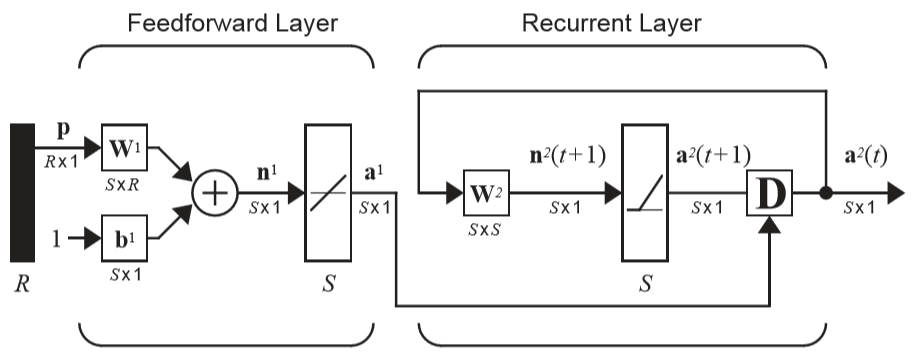
\includegraphics[width=16cm]{img/hamming/diagrama.png}
        \caption{Estructura de la red de Hamming. \cite{libro1}}
        \label{fig:hamming-diagrama2}
    \end{center}
\end{figure}
Para hacer la primera prueba sobre la red Hamming se utilizo el siguiente conjunto de vectores prototipo.
\[ \left\lbrace \boldsymbol{p_1} = \left[\begin{array}{c}-1\\ 1\\ -1\end{array}\right], \boldsymbol{p_2} = \left[\begin{array}{c}-1\\ -1\\ 1\end{array}\right], \boldsymbol{p_3} = \left[\begin{array}{c}1\\ 1\\ -1\end{array}\right], \boldsymbol{p_4} = \left[\begin{array}{c}1\\ -1\\ -1\end{array}\right] \right\rbrace \]
Y el vector de a clasificar fue el siguiente.
\[ \boldsymbol{p} = \left[\begin{array}{c}-1\\ 1\\ -1\end{array}\right] \]
Por lo que la arquitectura definida en la figura \ref{fig:hamming-diagrama2} tiene los siguientes valores.
\begin{align*}
R = 3 \implies \boldsymbol{b^1} = \left[\begin{array}{c}3\\ 3\\ 3\end{array}\right] && S = 4 && \boldsymbol{W^1} = \left[\begin{array}{c}\boldsymbol{p^{T}_1}\\ \boldsymbol{p^{T}_2}\\ \boldsymbol{p^{T}_3} \\ \boldsymbol{p^{T}_4}\end{array}\right]
\end{align*}
Al aplicar estos valores a nuestra red la capa recurrente termino en la iteración 13 y convergió exitosamente a la clase 1 que es la que se esperaba que convergiera.
%modelo matemático, arquitectura, conjunto de entrenamiento, condición de finalización, valores finales de w y bias
\begin{figure}[H]
    \begin{center}
        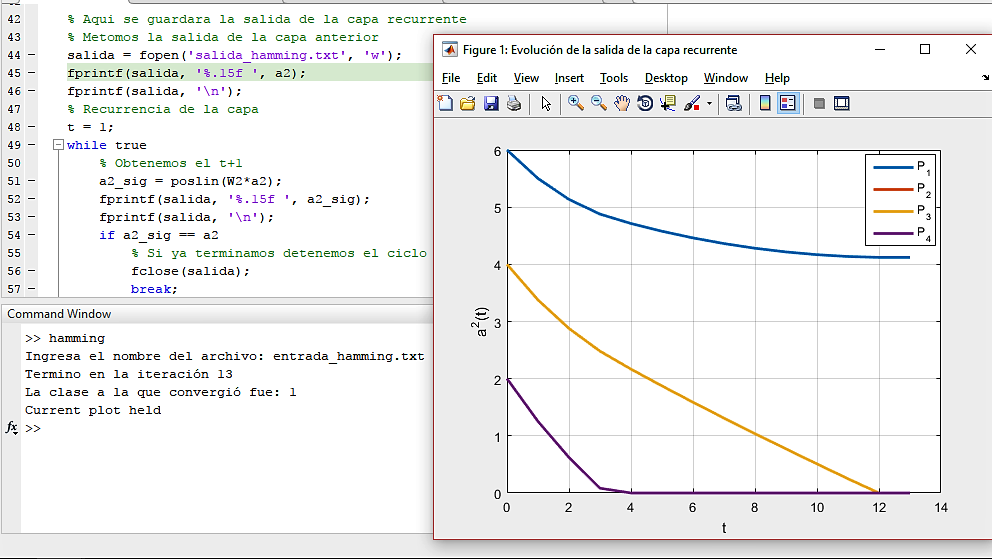
\includegraphics[width=16cm]{img/hamming/hamming1.png}
        \caption{Prueba 1 de la red Hamming.}
        \label{fig:hamming1}
    \end{center}
\end{figure}
En la figura \ref{fig:hamming1} se puede observar que solo la curva asociada a la neurona 1 de la capa recurrente que corresponde al vector prototipo 1 es la única que tiene un valor distinto de 0.
\newline
\textbf{Experimento 2.}
En esta segunda prueba se utilizo el siguiente conjunto de vectores prototipo.
\[ \left\lbrace \boldsymbol{p_1} = \left[\begin{array}{c}1\\ -1\\ -1 \\ -1 \end{array}\right], \boldsymbol{p_2} = \left[\begin{array}{c}-1\\ -1\\ -1 \\ 1 \end{array}\right] \right\rbrace \]
El vector de prueba a clasificar fue el siguiente.
\[ \boldsymbol{p} = \left[\begin{array}{c}1\\ 1\\ -1 \\ -1\end{array}\right] \]
Los valores fueron ingresados mediante un archivo de texto llamado \emph{entrada\_hamming2.txt}. Esto dio como resultado que los valores de la red Hamming de la figura \ref{fig:hamming-diagrama2} sean los siguientes.
\begin{align*}
R = 4 \implies \boldsymbol{b} = \left[\begin{array}{c}4 \\4\end{array}\right] && S = 2 && \boldsymbol{W} = \left[\begin{array}{c}\boldsymbol{p^{T}_1}\\ \boldsymbol{p^{T}_2}\end{array}\right]
\end{align*}
\begin{figure}[H]
    \begin{center}
        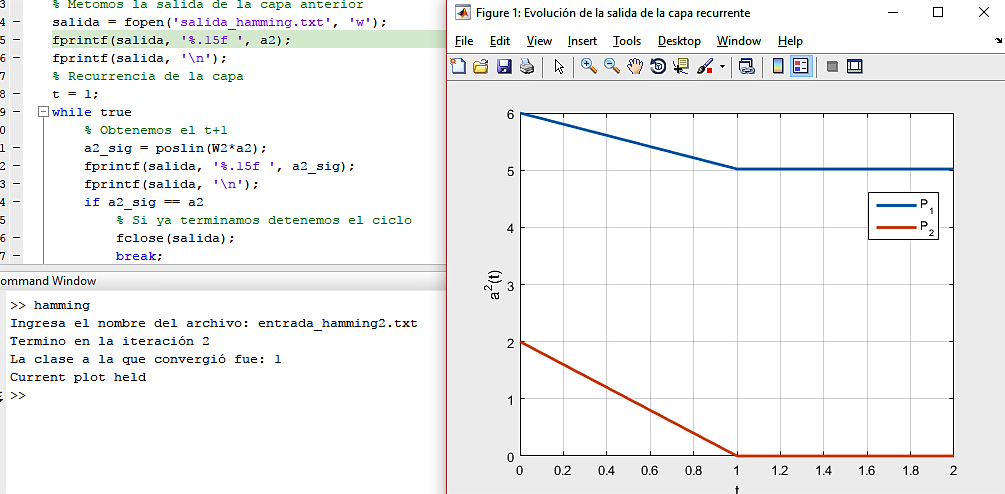
\includegraphics[width=16cm]{img/hamming/hamming2.png}
        \caption{Prueba 2 de la red Hamming.}
        \label{fig:hamming2}
    \end{center}
\end{figure}
Después del procesamiento de estos datos se pudo clasificar correctamente el vector de entrada, a la red le tomo dos iteraciones logar converger y a la clase a la que convergió fue la 1, esto se puede observar a detalle en la evolución de las salidas de la capa recurrente que se encuentra en la figura \ref{fig:hamming2}.
\newline
\textbf{Experimento 3.} En este ultimo experimento se utilizo un archivo llamado \emph{entrada\_hamming3.txt} para poder ingresar los datos a la red. El conjunto de vectores prototipo fue el siguiente.
\[ \left\lbrace \boldsymbol{p_1} = \left[\begin{array}{c}-1\\ 1\\ 1 \\ 1 \\ 1 \end{array}\right], \boldsymbol{p_2} = \left[\begin{array}{c}-1\\ -1\\ 1 \\ -1 \\ 1 \end{array}\right], \boldsymbol{p_3} = \left[\begin{array}{c}1\\ 1\\ -1 \\ -1 \\ -1 \end{array}\right], \boldsymbol{p_4} = \left[\begin{array}{c}-1\\ -1\\ -1 \\ -1 \\ -1 \end{array}\right], \boldsymbol{p_5} = \left[\begin{array}{c}1\\ 1\\ 1 \\ 1 \\ 1 \end{array}\right] \right\rbrace \]
El vector de prueba que se utilizo fue.
\[ \boldsymbol{p} = \left[\begin{array}{c}1\\ -1\\ 1 \\ -1 \\ 1\end{array}\right] \]
El utilizar estos valores produjo que la arquitectura de la figura \ref{fig:hamming-diagrama2} tuviera los siguientes valores.
\begin{align*}
R = 5 \implies \boldsymbol{b} = \left[\begin{array}{c}5 \\5 \\ 5 \\ 5 \\ 5\end{array}\right] && S = 5 && \boldsymbol{W} = \left[\begin{array}{c}\boldsymbol{p^{T}_1}\\ \boldsymbol{p^{T}_2} \\ \boldsymbol{p^{T}_3} \\ \boldsymbol{p^{T}_4} \\ \boldsymbol{p^{T}_5}\end{array}\right]
\end{align*}
\begin{figure}[H]
    \begin{center}
        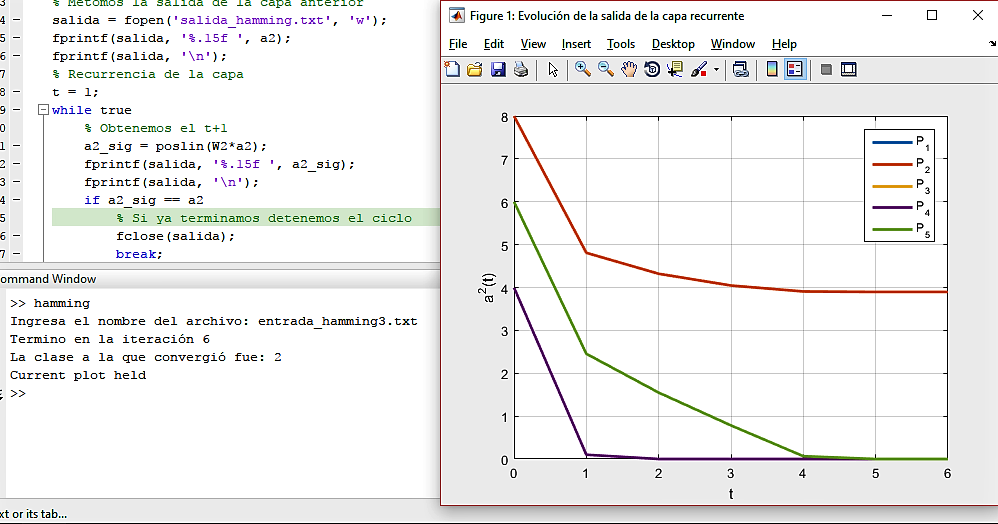
\includegraphics[width=16cm]{img/hamming/hamming3.png}
        \caption{Prueba 3 de la red Hamming.}
        \label{fig:hamming3}
    \end{center}
\end{figure}
Como se puede observar en la figura \ref{fig:hamming3} la red pudo converger a un resultado satisfactorio en la iteración 6 dando como resultado que el vector de prueba perteneciera a la clase 2 debido a que es la única salida que tiene un valor diferente a 0.
\newpage
    %\include{perceptron}
    \subsection{ADALINE}
        Los experimentos en ADALINE consistieron se dividieron en dos partes, la primera para pruebas que involucraran bias en donde se introdujo un archivo con el conjunto de entrenamiento al igual que en el perceptron, y por otro lado para la parte en la que no se utilizo el bias sólo se resolvió el problema del codificador en el cual el usuario indica el tamaño del codificador y la red comienza a trabajar como lo haría comúnmente.
        
        Ambos tipos de experimentos incluyen la graficación de la evolución del error por iteración y de los valores de pesos y bias, además de que los valores finales son almacenados en un archivo llamado \emph{resultado\_hora\_fecha.txt}
        \begin{figure}[H]
            \begin{center}
                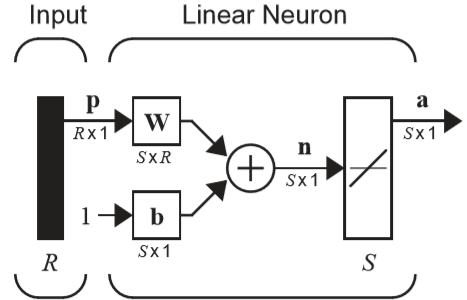
\includegraphics[width=9cm]{img/adaline/arquitectura.png}
                \caption{Arquitectura de la red ADALINE con bias. \cite{libro1}}
                \label{fig:adaline-diagrama2}
            \end{center}
        \end{figure}
            \subsubsection{Con bias}
            \textbf{Experimento 1}
            El conjunto de entrenamiento que se utilizo en este caso fue.
            \[ \left\lbrace \boldsymbol{p_1} = \left[\begin{array}{c} 0\\ 0\end{array}\right], t_1 = -1  \right\rbrace, \left\lbrace \boldsymbol{p_2} = \left[\begin{array}{c} 0\\ 1\end{array}\right], t_2 = -1  \right\rbrace, \left\lbrace \boldsymbol{p_3} = \left[\begin{array}{c} 1\\ 0\end{array}\right], t_3 = -1  \right\rbrace, \left\lbrace \boldsymbol{p_4} = \left[\begin{array}{c} 1\\ 1\end{array}\right], t_4 = 1  \right\rbrace  \]
            El cual corresponde a una compuerta AND de dos entradas. Esto provoco que los valores asociados a nuestra arquitectura de la figura \ref{fig:adaline-diagrama2} fueran los siguientes.
            \begin{align*}
                S=1 && R=2
            \end{align*}
            Además los valores asociados a $\boldsymbol{W}$ y $\boldsymbol{b}$ fueron números aleatorios pequeños. De igual forma se ingresan los valores para el factores de aprendizaje, número máximo de iteraciones y el mínimo error permitido, $\alpha=.03$, $it_{max}=100$, $e_{it}=.1$ respectivamente.
            \begin{figure}[H]
                \begin{center}
                    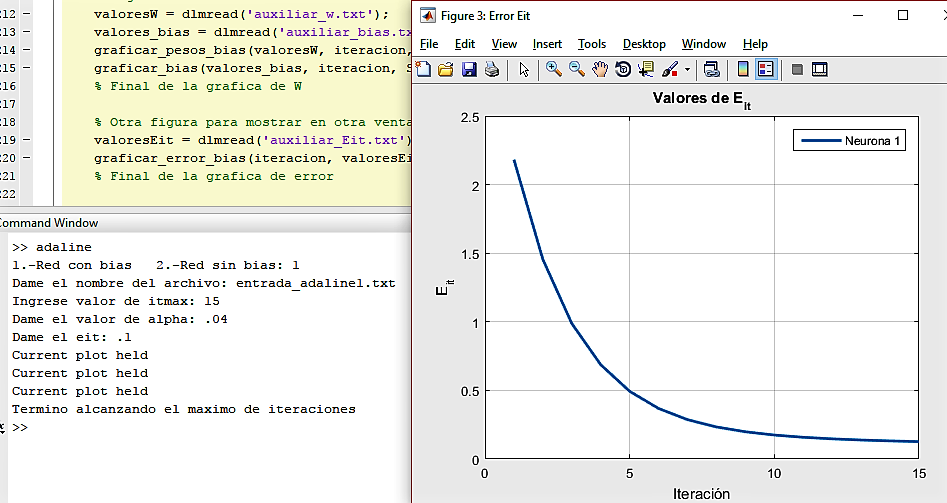
\includegraphics[width=16cm]{img/adaline1/error.png}
                    \caption{Prueba 1 de ADALINE con bias.}
                    \label{fig:adaline1error}
                \end{center}
            \end{figure}
            En la figura \ref{fig:adaline1error} se puede observar que la red llego a un resultado en la iteración 25 debido al criterio de error menor al permitido por iteración como se ve reflejado en la gráfica correspondiente, dando como resultado los siguientes valores para los pesos y bias.
            \begin{align*}
                \boldsymbol{W} = \left[\begin{array}{cc}0.5744 & 0.5956\end{array}\right] && \boldsymbol{b} = -0.9391
            \end{align*}
            Estos valores son almacenados en su respectivo archivo \emph{resultado\_hora\_fecha.txt}, en la figura \ref{fig:adaline1pesos} se puede observar su evolución a lo largo de las 25 iteraciones.
            \begin{figure}[H]
                \begin{center}
                    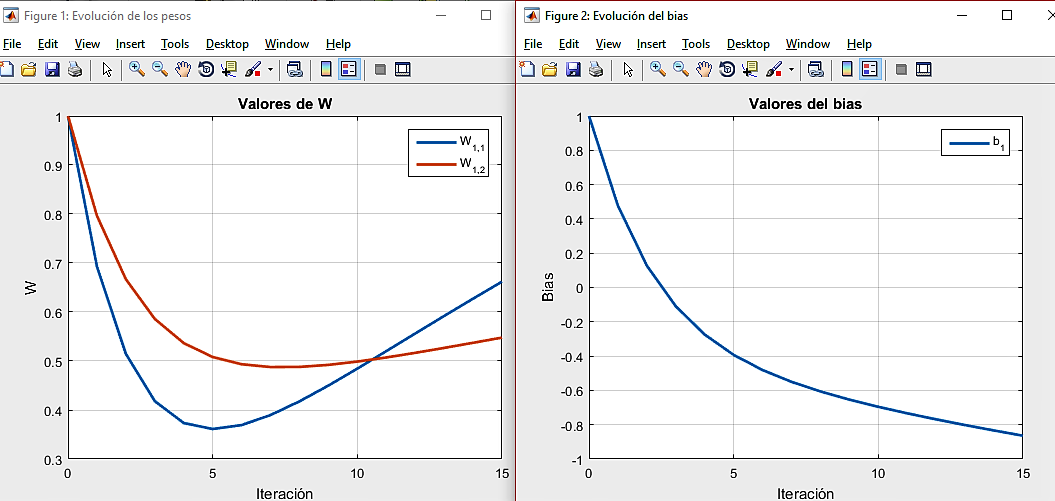
\includegraphics[width=16cm]{img/adaline1/pesosbias.png}
                    \caption{Pesos y bias en esta prueba.}
                    \label{fig:adaline1pesos}
                \end{center}
            \end{figure}
        \textbf{Experimento 2}
        El conjunto de entrenamiento que se utilizo para entrenar a la red fue.
        \[ \left\lbrace \boldsymbol{p_1} = \left[\begin{array}{c} 1\\ 1\end{array}\right], \boldsymbol{t_1} = \left[\begin{array}{c} -1\\ -1\end{array}\right]  \right\rbrace, \left\lbrace \boldsymbol{p_2} = \left[\begin{array}{c} 2\\ 0\end{array}\right], \boldsymbol{t_2} = \left[\begin{array}{c} -1\\ -1\end{array}\right]  \right\rbrace, \left\lbrace \boldsymbol{p_3} = \left[\begin{array}{c} -1\\ -1\end{array}\right], \boldsymbol{t_3} = \left[\begin{array}{c} -1\\ 1\end{array}\right]  \right\rbrace,\]
        
        \[ \left\lbrace \boldsymbol{p_4} = \left[\begin{array}{c} 0\\ -1\end{array}\right], \boldsymbol{t_4} = \left[\begin{array}{c} -1\\ 1\end{array}\right]  \right\rbrace, \left\lbrace \boldsymbol{p_5} = \left[\begin{array}{c} -2\\ 0\end{array}\right],\boldsymbol{t_5} = \left[\begin{array}{c} 1\\ -1\end{array}\right]  \right\rbrace, \left\lbrace \boldsymbol{p_6} = \left[\begin{array}{c} -1\\ 1\end{array}\right], \boldsymbol{t_6} = \left[\begin{array}{c} 1\\ -1\end{array}\right]  \right\rbrace,\]
        
        \[ \left\lbrace \boldsymbol{p_7} = \left[\begin{array}{c} 0\\ 2\end{array}\right], \boldsymbol{t_7} = \left[\begin{array}{c} 1\\ 1\end{array}\right]  \right\rbrace, \left\lbrace \boldsymbol{p_8} = \left[\begin{array}{c} 1\\ 2\end{array}\right], \boldsymbol{t_8} = \left[\begin{array}{c} 1\\ 1\end{array}\right]  \right\rbrace\]
        Es por estos valores que las dimensiones de la red mostrada en la figura \ref{fig:adaline-diagrama2} quedan definidas de la siguiente forma.
        \begin{align*}
            S = 2 && R = 2
        \end{align*}
        Lo cual crea una matriz de pesos de $2x2$ y una matriz de bias de $2x1$ con valores aleatorios pequeños, mientras que los valores de iteración máxima, factor de aprendizaje y error permitido son de nueva cuenta introducidos manualmente de la forma $it_{max}=20$, $\alpha=0.04$,  $e_{it}=0.1$ respectivamente (véase figura \ref{fig:adaline2error}).
        \begin{figure}[H]
            \begin{center}
                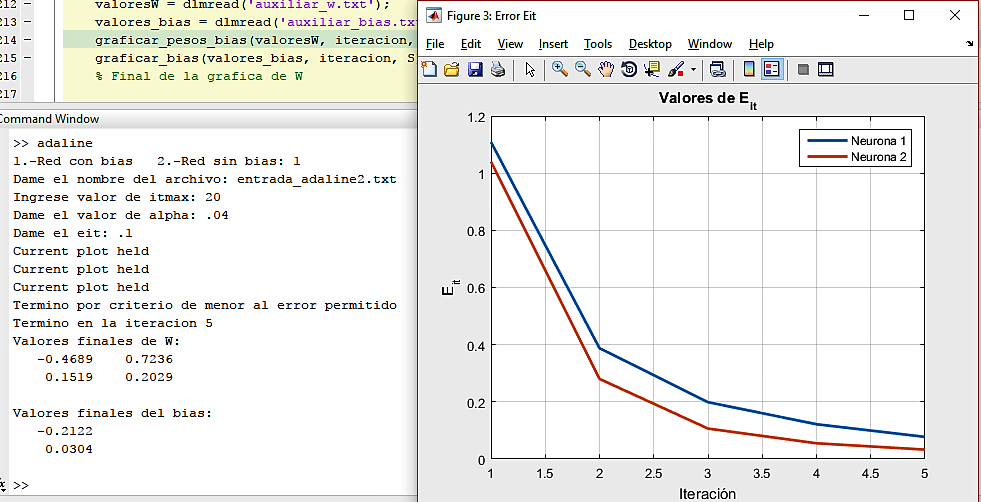
\includegraphics[width=16cm]{img/adaline2/error.png}
                \caption{Prueba 2 de ADALINE con bias.}
                \label{fig:adaline2error}
            \end{center}
        \end{figure}
        En esta ocasión la red convergió en la iteración 5 debido al criterio de menor al error permitido reflejado en la figura \ref{fig:adaline2error} para cada una de las neuronas que componen esta red. Los valores finales de pesos y bias se almacenaron en su correspondiente archivo de salida con los valores.
        \begin{align*}
            \boldsymbol{W} = \left[\begin{array}{cc}-0.4648& 0.7236\\ 0.1519& 0.2029\end{array}\right] && \boldsymbol{b} = \left[\begin{array}{c}-0.2122\\ 0.0304\end{array}\right]
        \end{align*}
        \begin{figure}[H]
            \begin{center}
                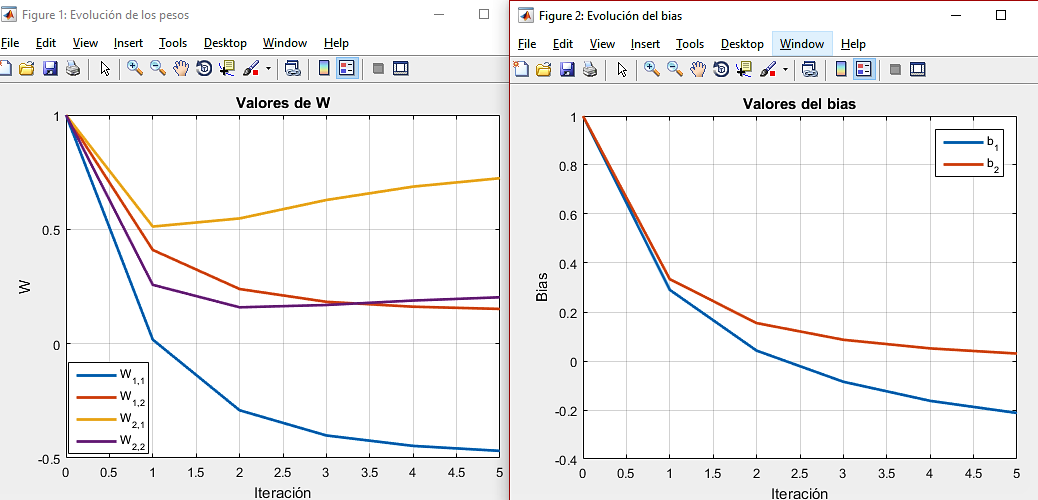
\includegraphics[width=16cm]{img/adaline2/pesosbias.png}
                \caption{Pesos y bias en esta prueba.}
                \label{fig:adaline2pesos}
            \end{center}
        \end{figure}
            \subsubsection{Sin bias}
            \textbf{Experimento 1}. En este caso el tamaño del codificador ingresado por el usuario fue de 4, el error mínimo aceptable fue $e_{it} = 0.01$ y el valor de alpha fue $\alpha=0.02$, esto se puede observar en la figura \ref{fig:adaline3error}.
            \begin{figure}[H]
                \begin{center}
                    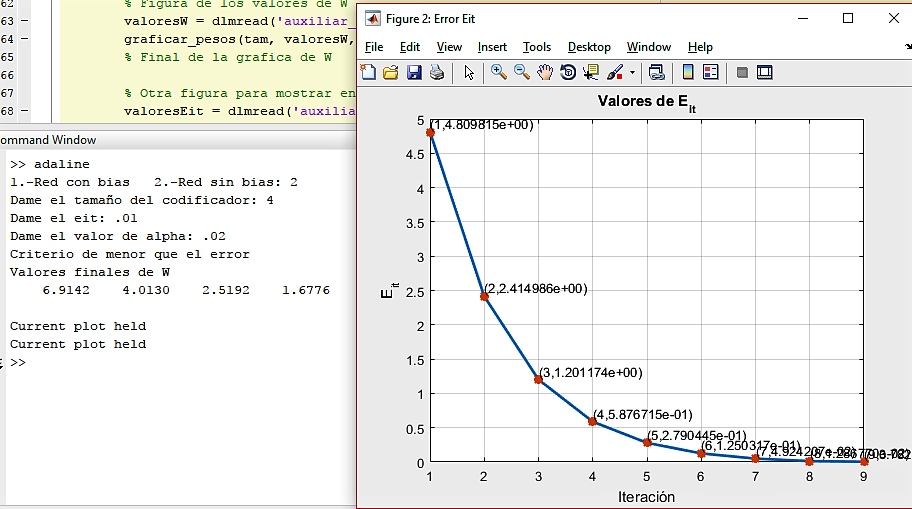
\includegraphics[width=16cm]{img/adaline3/error.png}
                    \caption{Prueba 1 de ADALINE sin bias.}
                    \label{fig:adaline3error}
                \end{center}
            \end{figure}
            La red convergió en la debido a que el error es menor al valor aceptable dando como resultado los siguientes valores de $\boldsymbol{W}$.
            \[ \boldsymbol{W} = \left[\begin{array}{cccc}6.9142 & 4.0130 & 2.5192 & 1.6776\end{array}\right] \]
            \begin{figure}[H]
                \begin{center}
                    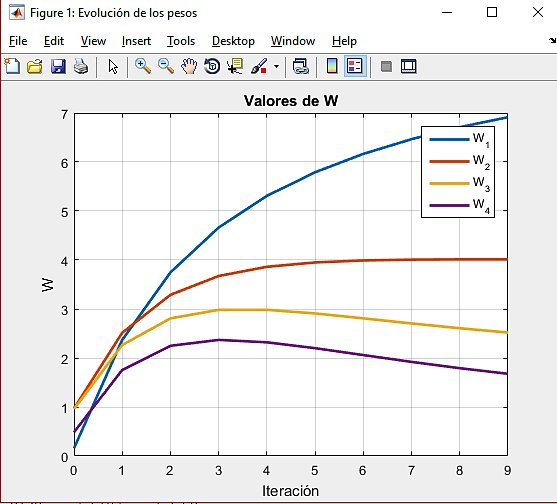
\includegraphics[width=10cm]{img/adaline3/pesosbias.png}
                    \caption{Pesos de esta prueba.}
                    \label{fig:adaline3pesos}
                \end{center}
            \end{figure}
        \textbf{Experimento 2}. En este caso el tamaño del codificador ingresado por el usuario fue de 5, el error mínimo aceptable fue $e_{it} = 0.01$ y el valor de alpha fue $\alpha=.03$, esto se puede observar en la figura \ref{fig:adaline4error}
        \begin{figure}[H]
            \begin{center}
                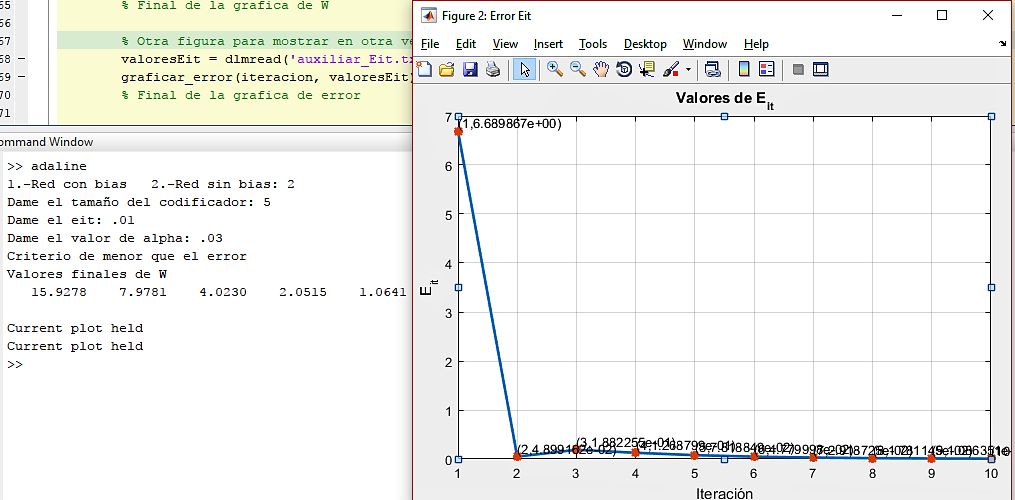
\includegraphics[width=16cm]{img/adaline4/error.png}
                \caption{Prueba 2 de ADALINE sin bias.}
                \label{fig:adaline4error}
            \end{center}
        \end{figure}
        La red convergió en la debido a que el error es menor al valor aceptable dando como resultado los siguientes valores de $\boldsymbol{W}$.
        \[ \boldsymbol{W} = \left[\begin{array}{ccccc}15.9278 & 7.9781 & 4.023 & 2.0515 & 1.0641\end{array}\right] \]
        \begin{figure}[H]
            \begin{center}
                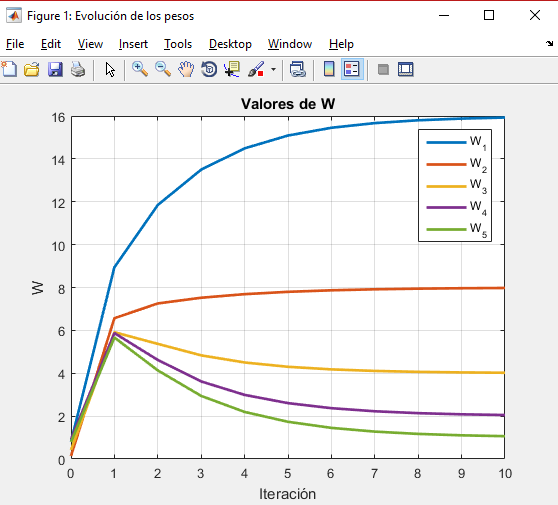
\includegraphics[width=10cm]{img/adaline4/pesosbias.png}
                \caption{Pesos de esta prueba.}
                \label{fig:adaline4pesos}
            \end{center}
        \end{figure}
    \section{Discusión de resultados}
\subsection{Hamming}
\subsection{Perceptron}
\subsection{ADALINE}
    \section{Conclusiones}
Sin duda alguna el perceptrón multicapa es una herramienta sumamente poderosa no por nada es la arquitectura más utilizada actualmente, esta práctica solo es una muestra de ello debido a que solo se utilizo para la aproximación de funciones. Sin embargo, es importante tener en cuenta que para su correcto funcionamiento se deben considerar diversos factores.

Dichos factores afectaron a la elaboración de esta práctica como el hecho de no tener tantos datos como ocurrió en el primer experimento realizado. Otra cuestión que es importante mencionar es que el tiempo de ejecución puede llegar a ser bastante alto por lo que contar con un buen hardware es de suma importancia, en este caso los tiempos alcanzaron casi 10 minutos para la máxima cantidad de datos y 5000 iteraciones. Lo cual puede parecer poco tiempo pero si se tratara de usar en un ambiente real se puede llegar a trabajar con millones de datos por lo cual no seria de utilidad, dicho problema se podría solucionar al utilizar otro lenguaje de programación más rápido como es el caso de C.

Finalmente, es evidente que se puede mejorar el entrenamiento utilizando valores de pesos, bias y factor de aprendizaje más específicos por lo que seria de gran utilidad tener un pre procesamiento de los datos que genere mejores valores de dichos parámetros y no solo utilizar valores aleatorios.
    \bibliographystyle{apalike}
    \bibliography{bibliografia}
    %    \section{Anexo}
        En esta sección se encuentra el código de los tres programas desarrollados en MATLAB.
        \subsection{Hamming}
        \begin{lstlisting}
% Cada elemento del vector de entrada tiene solo dos posibles valores
opcion = input('Ingresa el nombre del archivo: ', 's');
archivo = dlmread(opcion);
tam = size(archivo);
% Tam de nuestros vectores prototipo
R = tam(2);

% Numero de neuronas, corresponde a cada vector prototipo
S = tam(1) - 1;

% Vector a clasificar
p = archivo(S+1, :)';

% Las filas de W1 son los vectores prototipos
% Inicializacion de W1
W1 = archivo(1:S, :);

% Cada elemento del bias es el tam del vector prototipo
% Inicializacion del bias
b1 = ones(S, 1) * R;

% Propagamos hacia adelante
a1 = purelin((W1*p)+b1);
% Fin de la capa feedforward

%Inicio de la capa recurrente
a2 = a1;
% Obtencion del valor epsilon 0 < epsilon < 1/(S-1)
epsilon = round(rand(1)*1/(S-1), 4); 
% Inicializacion y llenado de la W2 de la capa recurrente
W2 = ones(S, S);
for i = 1:S
    for j = 1:S
        if i==j
            W2(i, j) = 1;
        else
            W2(i, j) = -epsilon; 
        end;
    end;
end;

% Aqui se guardara la salida de la capa recurrente
% Metomos la salida de la capa anterior
salida = fopen('salida_hamming.txt', 'w');
fprintf(salida, '%.15f ', a2);
fprintf(salida, '\n');
% Recurrencia de la capa
t = 1;
while true
    % Obtenemos el t+1
    a2_sig = poslin(W2*a2);
    fprintf(salida, '%.15f ', a2_sig);
    fprintf(salida, '\n');
    if a2_sig == a2
        % Si ya terminamos detenemos el ciclo
        fclose(salida);
        break;
    else
        % Siguiente iteracion
        a2 = a2_sig;
    end;
    t = t + 1;
end;

% Fin de la capa recurrente
fprintf('Termino en la iteracion %d\n', t);
v = 1;
for ite = a2'
    if ite ~= 0
        break;
    else
        v = v+1;
    end;
end
fprintf('La clase a la que convergio fue: %d\n', v);
% Imprimir datos y graficar la salida de a2
a2_recurrente = dlmread('salida_hamming.txt');
figure('Name', 'Evolucion de la salida de la capa recurrente');
plot(0:t, a2_recurrente, 'LineWidth', 2);
hold;
grid;
xlabel('t');
ylabel('a^2(t)');
etiquetas = cell(1, S);
for i = 1:S
    etiquetas{i} = ['P_' num2str(i)];
end;
legend(etiquetas);
        \end{lstlisting}
        \subsection{Perceptron}
        \subsection{ADALINE}
        \begin{lstlisting}
%% Funcion principal
function adaline()
    opcion = input('1.-Red con bias   2.-Red sin bias: ', 's');
    if str2double(opcion) == 1
        adaline_bias();
    else
        % Captura de los datos
        tam = input('Dame el tam del codificador: ', 's');
        tam = str2double(tam);
        tabla_verdad = zeros(2^tam, tam+1);
        eit = input('Dame el eit: ', 's');
        eit = str2double(eit);
        alpha = input('Dame el valor de alpha: ', 's'); % 0.3
        alpha = str2double(alpha);
        N = 2^tam-1;
        W = rand(1, tam);
        auxiliar_w = fopen('auxiliar_w.txt', 'w');
        auxiliar_Eit = fopen('auxiliar_Eit.txt', 'w');
        fprintf(auxiliar_w, '%.10f ', W);
        fprintf(auxiliar_w, '\n');
        % Llenamos nuestra tabla de verdad
        for i = 0:N
            a = dec2bin(i, tam) - '0';
            tabla_verdad(i+1, 1:tam) = a;
            tabla_verdad(i+1, tam+1) = i;
        end;
        continuar = true;
        iteracion = 1;
        while continuar
            Eit = 0;
            for n = 1:N
                p = tabla_verdad(n, 1:tam)';
                a = purelin(W*p);
                t = tabla_verdad(n, tam+1);
                ed = t-a;
                Eit = Eit + ed;
                W = W + (2 * alpha * ed*p');
            end
            Eit = 1/N * Eit;
            Eit = abs(Eit);
            fprintf(auxiliar_Eit, '%.10f ', Eit);
            fprintf(auxiliar_Eit, '\n');
        
            fprintf(auxiliar_w, '%.10f ', W);
            fprintf(auxiliar_w, '\n');
            if Eit == 0
                disp('Criterio de igualdad a cero');
                break;
            elseif Eit < eit
                disp('Criterio de menor que el error');
                break;
            end
            iteracion = iteracion + 1;
        end
        fclose(auxiliar_Eit);
        fclose(auxiliar_w);
    
        % Desplegar los valores finales
        disp('Valores finales de W');
        disp(W);
        
        % Figura de los valores de W
        valoresW = dlmread('auxiliar_w.txt');
        graficar_pesos(tam, valoresW, iteracion);
        % Final de la grafica de W
        
        % Otra figura para mostrar en otra ventana
        valoresEit = dlmread('auxiliar_Eit.txt');
        graficar_error(iteracion, valoresEit)
        % Final de la grafica de error
        
        % Guardamos en un archivo
        a_final = strcat('resultado_', datestr(now, 'HH-MM_dd-mm-yyyy'));
        a_final = strcat(a_final, '.txt');
        valores_finales = fopen(a_final, 'w');
        fprintf(valores_finales, 'Valores finales de W \n');
        fprintf(valores_finales, '%.10f ', W);
        fprintf(valores_finales, '\n');
        fclose(valores_finales);
    end
end % Final de la funcion principal

%% graficar_pesos: function description
function graficar_pesos(tam, valoresW, iteracion)
    figure('Name', 'Evolucion de los pesos');
    % Grafica un vector en x y otro vector en y
    plot(0:iteracion, valoresW, 'LineWidth', 2); 
    hold;
    grid;
    % Etiquetas de los ejes
    xlabel('Iteracion');
    ylabel('W');
    
    % Titulo de nuestra grafica
    etiquetas = cell(1, tam);
    for i = 1:tam
        etiquetas{i} = ['W_' num2str(i)];
    end;
    legend(etiquetas);
    title('Valores de W');
end

%% graficar_error: function description
function graficar_error(iteracion, valoresEit)
    figure('Name', 'Error Eit');
    x = 1:iteracion;
    % Grafica un vector en x y otro vector en y
    plot(x, valoresEit, 'LineWidth', 2);
    hold;
    plot(x, valoresEit, '*', 'LineWidth', 2);
    grid;
    % Imprime las coordenadas de Eit
    strValues = strtrim(cellstr(num2str([x(:) valoresEit(:)], '(%d,%d)')));
    text(x, valoresEit, strValues, 'VerticalAlignment', 'bottom');
    % Etiquetas de los ejes
    xlabel('Iteracion');
    ylabel('E_{it}');
    % Titulo de nuestra grafica
    title('Valores de E_{it}');
end

%Con bias
function adaline_bias()
    archivo = input('Dame el nombre del archivo: ', 's');
    prueba = fopen(archivo, 'r');
    S = 0;
    targets = [];
    prototipos = [];
    R = 0;
    dimen = [];
    tipo_lectura = 0;
    while feof(prueba) == 0
        linea = fgetl(prueba);
        if linea ~= '{'
            fclose(prueba);
            datos = dlmread(archivo);
            tam = size(datos);
            S = 1;
            prototipos = datos(:, 1:tam(2)-1)';
            dimen = size(prototipos);
            targets = datos(:, tam(2))';
            R = dimen(1);
            tipo_lectura = 1;
            break;
        else
            linea = linea(2:length(linea)-1);
            proto = linea(2:find(linea==',')-2);
            tar = linea(find(linea==',')+2:length(linea)-1);
            proto = str2num(proto);
            tar = str2num(tar);
            prototipos = [prototipos proto'];
            targets = [targets tar'];
        end
    end
    if tipo_lectura == 0
        S = 2;
        dimen = size(prototipos);
        R = dimen(1);
    end   
    itmax = input('Ingrese valor de itmax: ', 's'); %5
    itmax = str2double(itmax);
    alpha = input('Dame el valor de alpha: ', 's'); % 0.3
    alpha = str2double(alpha);
    eit = input('Dame el eit: ', 's');
    eit = str2double(eit);
    W = ones(S, R);
    b = ones(S, 1);
    
    auxiliar_w = fopen('auxiliar_w.txt', 'w');
    auxiliar_bias = fopen('auxiliar_bias.txt', 'w');
    auxiliar_error = fopen('auxiliar_Eit.txt', 'w');
    fprintf(auxiliar_w, '%.10f ', W);
    fprintf(auxiliar_w, '\n');
    
    fprintf(auxiliar_bias, '%.10f ', b);
    fprintf(auxiliar_bias, '\n');
    criterio = 0;
    for iteracion = 1:itmax
        Eit = 0;
        for n = 1:dimen(2)
            p = prototipos(:, n);
            a = purelin(W*p + b);
            t = targets(:, n);
            ed = t-a;
            Eit = Eit + ed;
            W = W + (2 * alpha * ed * p');
            b = b + (2 * alpha * ed);
        end
        Eit = 1/dimen(2) * Eit;
        Eit = abs(Eit);
        fprintf(auxiliar_error, '%.10f ', Eit);
        fprintf(auxiliar_error, '\n');
        
        fprintf(auxiliar_w, '%.10f ', W);
        fprintf(auxiliar_w, '\n');
        
        fprintf(auxiliar_bias, '%.10f ', b);
        fprintf(auxiliar_bias, '\n');
        if Eit == 0
            criterio = 1;
            break;
        elseif Eit < eit
            criterio = 2;
            break;
        end
    end
    fclose(auxiliar_error);
    fclose(auxiliar_w);
    fclose(auxiliar_bias);
    
    % Figura de los valores de W
    valoresW = dlmread('auxiliar_w.txt');
    valores_bias = dlmread('auxiliar_bias.txt');
    graficar_pesos_bias(valoresW, iteracion, S, R);
    graficar_bias(valores_bias, iteracion, S);
    % Final de la grafica de W
    
    % Otra figura para mostrar en otra ventana
    valoresEit = dlmread('auxiliar_Eit.txt');
    graficar_error_bias(iteracion, valoresEit, S);
    % Final de la grafica de error
    
    if criterio == 0
        disp('Termino alcanzando el maximo de iteraciones')
    elseif criterio == 1
        disp('Termino por criterio de error igual a 0');
        fprintf('Termino en la iteracion %d\n', iteracion);
        disp('Valores finales de W:');
        disp(W);
        disp('Valores finales del bias:');
        disp(b);
    else
        disp('Termino por criterio de menor al error permitido');
        fprintf('Termino en la iteracion %d\n', iteracion);
        disp('Valores finales de W:');
        disp(W);
        disp('Valores finales del bias:');
        disp(b);
    end
    
    archivo_final = strcat('resultado_', datestr(now, 'HH-MM_dd-mm-yyyy'));
    archivo_final = strcat(archivo_final, '.txt');
    finales = fopen(archivo_final, 'w');
    fprintf(finales, 'Valores finales de W: \n');
    fprintf(finales, '%.10f ', W);
    fprintf(finales, '\n');
    
    fprintf(finales, 'Valores finales del bias: \n');
    fprintf(finales, '%.10f ', b);
    fprintf(finales, '\n');
    fclose(finales);
end


%% graficar_pesos: function description
function graficar_pesos_bias(valoresW, iteracion, S, R)
    figure('Name', 'Evolucion de los pesos');
    % Grafica un vector en x y otro vector en y
    plot(0:iteracion, valoresW, 'LineWidth', 2); 
    hold;
    grid;
    % Etiquetas de los ejes
    xlabel('Iteracion');
    ylabel('W');
    
    etiquetas = cell(1, S*R);
    k = 1;
    for i = 1:S
        for j = 1:R
            etiquetas{k} = ['W_{' num2str(i) ',' num2str(j) '}'];
            k = k+1;
        end;
    end;
    legend(etiquetas);
    title('Valores de W');
end

%% graficar_error: function description
function graficar_error_bias(iteracion, valoresEit, S)
    figure('Name', 'Error Eit');
    x = 1:iteracion;
    % Grafica un vector en x y otro vector en y
    plot(x, valoresEit, 'LineWidth', 2);
    hold;
    grid;
    % Etiquetas de los ejes
    xlabel('Iteracion');
    ylabel('E_{it}');
    % Titulo de nuestra grafica
    etiquetas = cell(1, S);
    for i = 1:S
        etiquetas{i} = ['Neurona ' num2str(i)];
    end;
    legend(etiquetas);
    % Titulo de nuestra grafica
    title('Valores de E_{it}');
end

%% graficar_bias
function graficar_bias(valores_bias, iteracion, S)
    figure('Name', 'Evolucion del bias');
    % Grafica un vector en x y otro vector en y
    plot(0:iteracion, valores_bias, 'LineWidth', 2); 
    hold;
    grid;
    % Etiquetas de los ejes
    xlabel('Iteracion');
    ylabel('Bias');
    % Titulo de nuestra grafica
    etiquetas = cell(1, S);
    for i = 1:S
        etiquetas{i} = ['b_' num2str(i)];
    end;
    legend(etiquetas);
    title('Valores del bias');
end
        \end{lstlisting}
\end{document}